\documentclass[12pt]{article}
\usepackage[toc,page]{appendix}
\usepackage{amsmath}
\usepackage{cases}
\usepackage{amsfonts}
\usepackage{epsfig}
\usepackage{setspace}
\usepackage{lscape}
\usepackage{natbib}
\usepackage{placeins}
\usepackage{epigraph}
\usepackage{verbatim}
\usepackage{epigraph}
\usepackage{url}
\usepackage{multirow}
\usepackage{rotating}
\usepackage[table]{xcolor}
\usepackage{graphicx}
\usepackage{caption}
\usepackage{subcaption}
\usepackage{nameref}
\DeclareMathOperator*{\E}{\mathbb{E}}
\bibliographystyle{agsm}
\usepackage{tikz}
\usepackage[colorlinks=true, linkcolor=blue]{hyperref}
%\citationstyle{dcu}
%\citationstyle{chicago}
%\bibliographystyle{harvard}
%\bibliographystyle{apalike}
%\usepackage{rotating}
\special{papersize=8.5in,11in}

\addtolength{\oddsidemargin}{-.5in} \addtolength{\evensidemargin}{-.5in}
\addtolength{\textwidth}{1in}

\addtolength{\topmargin}{-.5in} \addtolength{\textheight}{1in}

\makeatletter
\def\@sect#1#2#3#4#5#6[#7]#8{\ifnum #2>\c@secnumdepth
     \let\@svsec\@empty\else
     \refstepcounter{#1}\edef\@svsec{\csname the#1\endcsname. \hskip 0.4em}\fi
     \@tempskipa #5\relax
      \ifdim \@tempskipa>\z@
        \begingroup #6\relax
          \@hangfrom{\hskip #3\relax\@svsec}{\interlinepenalty \@M #8\par}%
        \endgroup
       \csname #1mark\endcsname{#7}\addcontentsline
         {toc}{#1}{\ifnum #2>\c@secnumdepth \else
                      \protect\numberline{\csname the#1\endcsname}\fi
                    #7}\else
        \def\@svsechd{#6\hskip #3\relax  %% \relax added 2 May 90
                   \@svsec #8\csname #1mark\endcsname
                      {#7}\addcontentsline
                           {toc}{#1}{\ifnum #2>\c@secnumdepth \else
                             \protect\numberline{\csname the#1\endcsname}\fi
                       #7}}\fi
     \@xsect{#5}}
\makeatother

\makeatletter
\renewcommand{\section}{\@startsection{section}{1}{0mm}{-\baselineskip}{0.25\baselineskip}{\centering\normalfont\normalsize\scshape}}
\renewcommand{\subsection}{\@startsection{subsection}{2}{0mm}{-\baselineskip}{0.25\baselineskip}{\raggedright\normalfont\normalsize\scshape}}
\renewcommand{\subsubsection}{\@startsection{subsubsection}{3}{0mm}{-\baselineskip}{0.25\baselineskip}{\raggedright\normalfont\small\scshape}}
\def\@begintheorem#1#2{\trivlist \item[\hskip \labelsep{\bf #1\ #2:}]\it}
\makeatother

\makeatletter
\def\monthname{\ifcase\month\or
January\or February\or March\or April\or May\or June\or July\or August\or
September\or October\or November\or December\fi} \makeatother

\renewenvironment{epigraphwidth}{\setlength{13.5cm}}

\renewcommand{\thesection}{\Roman{section}}
\renewcommand{\thesubsection}{\Alph{subsection}}

\renewenvironment{abstract}
 {\begin{center}\normalsize\textsc{}%
 \end{center}\begin{quote}\normalsize}
 {\end{quote}}


\renewcommand{\appendix}{\footnotesize\parindent 0cm\setlength{\parskip}{\medskipamount}\setcounter{equation}{0}%
\renewcommand{\theequation}{A.\arabic{equation}}}

\newtheorem{theorem}{\small\sc Theorem}[section]
\newtheorem{proposition}{\small\sc Proposition}[section]
\newtheorem{assumption}{\small\sc Assumption}[section]
\newtheorem{lemma}{\small\sc Lemma}[section]
\newtheorem{corollary}{\small\sc Corollary}[section]

\newcommand{\indep}{\perp\!\!\!\!\perp}

\begin{document}
%\begin{titlepage}
%\vspace*{0.2cm}
%
%\setcounter{page}{0}
%%\vskip 30pt
%\vskip 10pt
%  \begin{center}%
%    {\Large \sc Never Let a Good Crisis Go to Waste:\\ Agenda Setting and Legislative Voting \\ in Response to External Shocks
%   \vspace{.5cm} \par}%
%
%    \vskip 1em%
%    {\large
%     \lineskip .75em%
%      \begin{tabular}[t]{c}%
%       Jack Blumenau
%      \end{tabular}  
%\vskip 1em 
%\textsc{London School of Economics}
%\par}%
%      \vskip 2.5em%
%  \end{center}\par
%
% \vskip 3.0em
%\begin{center} \textsc{Abstract} \end{center}
%
%\begin{abstract}
%\end{abstract}
%
%
%
%
%
%\vfill
%  \footnoterule
%    {\footnotesize
%\noindent 	
%	This version: \monthname \ \number\year. \\
%
%
%\noindent\footnotesize
%
%}
%\end{titlepage}

\section*{Do party leader approval ratings predict election outcomes?}
\emph{Note: This piece \href{http://blogs.lse.ac.uk/generalelection/party-leader-approval-ratings-and-election-outcomes/}{originally featured} on the LSE general election blog, February 17, 2015}
\\~\\
\setcounter{page}{1} \addtolength{\baselineskip}{0.5\baselineskip}
\noindent A significant amount of attention is given to opinion polls measuring the popularity of party leaders. The implication of much of this coverage is that the approval of party leaders matters when voters cast their votes. While photos of leaders struggling to eat sandwiches, or wearing inappropriate holiday attire, may make for good copy, what evidence is there to suggest that the popularity of party leaders is consequential for election outcomes? %In this post, Jack Blumenau examines past trends in party leader approval, putting recent figures into historical context. He shows that leader approval ratings are much more volatile than general election vote shares, and that focusing solely on party leader approval leads to overly pessimistic predictions for the largest parties, and particularly for Labour.

Figure \ref{partysat} shows the trends in Labour, Conservative, and Liberal Democrat party leader net satisfaction from 1974 up until last week. Respondents are asked whether they are ``satisfied or dissatisfied with the way [a given party leader] is doing his/her job''. Net satisfaction is the proportion of respondents answering ``satisfied'' minus the proportion of respondents answering ``dissatisfied''. The data comes from Ipsos MORI's monthly political barometer surveys. Translucent points in the plot are the figures calculated from each survey, and the lines show the smoothed trend over time.


\begin{figure}
\begin{center}
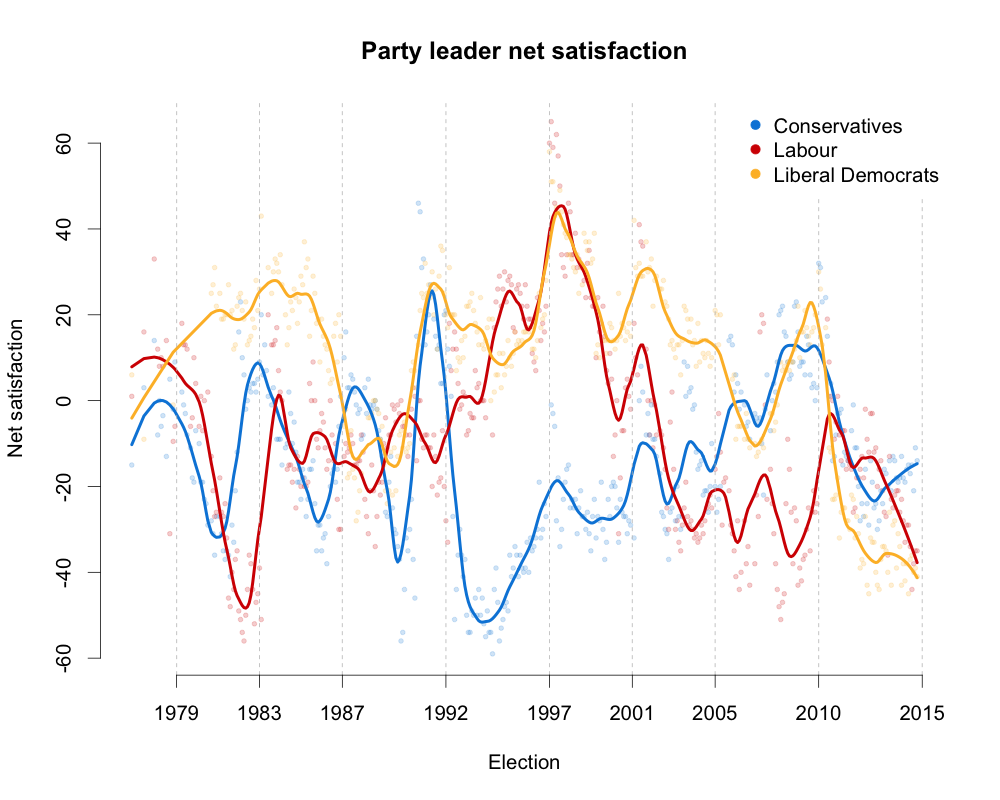
\includegraphics[width=\textwidth]{PartyLeaderSatisfaction.png}
\caption{Party leader net satisfaction over time}\label{partysat}
%\caption{Examples of $\varphi$}
\end{center}
\end{figure}


There are a few messages to take from this plot. First, collectively, today's leaders are an unpopular bunch. The average net rating of the main three party leaders is lower now than at any point since 1974.

Second, Ed Miliband's approval ratings are low, but not exceptional: both Michael Foot and Gordon Brown hit similar lows during their tenures. That said, given the subsequent electoral performance of Brown and Foot, this comparison is probably not much comfort to the Labour leader. Nick Clegg comes off particularly poorly when compared to the historical trend: the Lib Dem leader's average net approval rating since May 2010 is 44 points lower than the party's long-run average prior to the formation of the coalition. David Cameron, by contrast, can take some solace from this plot: the Conservative leader's current approval rating is comparable to the long-run average of his party, and 3 points higher than the average of previous Conservative prime ministers (a little lower than Thatcher, a little higher than Major).

Third, the approval of party leaders is negatively related to government participation. On average, across parties, leaders in government have approval ratings that are 17 points lower than leaders who are not in Downing Street. This is in line with the fact that electoral support for government parties tends to decrease in the middle of their terms of office. For example, John Major's approval rating plummeted after the Conservative election victory in 1992, while the popularity of Labour leaders increased until the election in 1997. After this point, net approval of Tony Blair decreased steadily throughout his prime ministerial tenure, while the popularity of Conservative leaders increased. More recently, the approval of both David Cameron and Nick Clegg decreased significantly after the formation of the coalition government in 2010. Notably, however, Ed Miliband has not followed the historic trend for opposition leaders. He is a little more unpopular now than Brown was at the end of his prime ministerial tenure.

The more relevant question, however, is whether any of this matters in terms of election outcomes. Does the (dis)approval of a party leader have any association with the share of the vote that a party receives? Figure \ref{predictions} shows the simplest possible model for predicting change in national vote share with changes in party leader approval. The x-axis shows the change in average party leader approval from the 100 days before one election to 100 days before the next election. The y-axis shows the change in national vote share from one election to the next. Each point represents a given party in a given election. The vertical lines are the predictions that this model produces for 2015. As there is substantial uncertainty in the relationship between party leader approval and vote share, these predictions are given as a range of plausible values (more technically, they represent the 90\% prediction intervals). The gray dashed line is the best-fitting line between these points.

\begin{figure}
\begin{center}
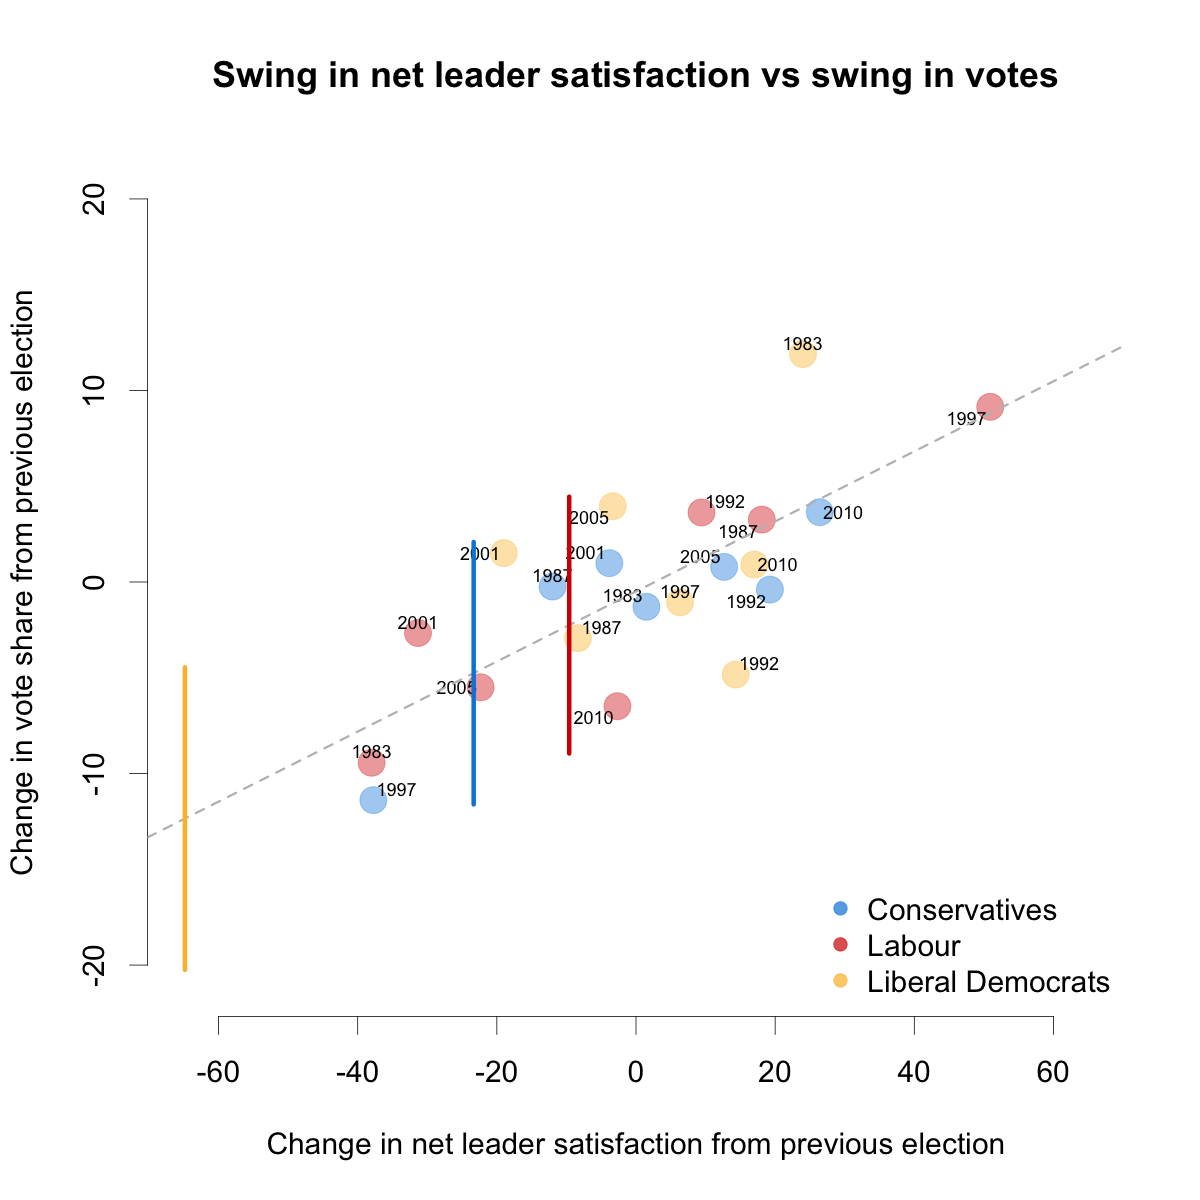
\includegraphics[width=\textwidth]{swing_vote_leader_pred.png}
%\caption{Examples of $\varphi$}
\caption{Predicted vote swing (2015) based on party leader approval ratings}\label{predictions}
\end{center}
\end{figure}

The plot shows that there is a relationship, but that it is not terribly strong. The main point is simple: party leaders' approval ratings fluctuate much more dramatically than parties' vote shares. A decline in a leader's personal net approval rating of 10 points, is associated with a decrease in vote share of only 2.3 percentage points. Overall, just because a party leader has become drastically unpopular, this does not mean that the party will lose a drastic number of votes at the election.

One interesting aspect of this analysis is that while Ed Miliband's current ratings are low in absolute terms, they are not much lower than Gordon Brown's were during the equivalent period in 2010. Because the model here focuses on \emph{change} in approval ratings, Labour's vote share is predicted to fall by only 2 percentage points. One interpretation of this is that voters in 2010 had already accounted for the fact that the Labour leader was unpopular, and so the unpopularity of Miliband in 2015 is unlikely to lead to (further) large declines in Labour's vote share in 2015. By contrast, because David Cameron was relatively popular prior to 2010, the model suggests that the Conservatives share of the national vote will decline more than the Labour share (by about 5 percentage points).

The plot suggests a particularly dire situation for the Liberal Democrats (a 12.3 percentage point fall in national vote share), but the model is possibly less informative for the Lib Dems. Their vote share has historically been less strongly associated with party leader approval than is the case for Labour and the Conservatives. We have also never witnessed a Lib Dem leader as unpopular as Nick Clegg. The upshot is that the extrapolation implied by this model almost certainly overestimates the extent of the Lib Dem demise in 2015, regardless of Clegg's current (woeful) personal ratings.

One way of assessing these party-leader based forecasts is to compare them to more sophisticated models of what might happen in May. For instance, the forecasts produced by the team at \href{http://electionforecast.co.uk}{electionforecast.co.uk} include estimates of the support for each party as the polls stand today. Comparing these forecasts reveals that the point estimates for the Conservatives and Liberal Democrats are slightly lower in the party leader model, though both models suggest that these parties will lose votes in 2015. For Labour, on the other hand, the election forecast model suggests that the polls currently have Labour increasing their vote share by about two and a half percentage points, relative to 2010, whereas the party leader model suggests that Labour will lose votes. However, there is substantial uncertainty in the relationship between leader approval and vote shares (evidenced by the fact that the prediction intervals cover a very wide range of changes in vote share), and the uncertainty intervals for all three parties include the the electionforecast predictions.

Some caveats: this is probably not a very good model. Not only is the uncertainty associated with the predictions very large, the analysis only takes into account the relative change in party leader approval from one election to the next, and does not account for any of the other factors that might be associated with changes in vote share in UK elections. Additionally, the model does not suggest that this relationship is causal: party leader approval may determine vote choice, or voters' more generic party evaluations may influence how they view party leaders. Likewise, it may be that myriad other factors � the state of the economy; which policy issues are currently salient; how parties other than the historical ``top-three'' are faring � drive both party leader approval and national vote shares.

The analysis simply reveals that if we were to use party leader approval as the only basis for predicting election outcomes, we would produce 2015 forecasts that are broadly consistent with other approaches. However, if we were to use this model for predictive purposes, such an analysis would lead to conclusions that are overly pessimistic for the main three parties, and particularly for the Labour Party.
\\~\\
\emph{Note: Only party leaders from Labour, the Conservatives, and the Liberal Democrats are analysed here. Prior to 1989 I consider David Steel to be the leader of the Liberals. Results are unaffected by including Roy Jenkins or David Owen from the SDP.}

\end{document}
